% This procedure has three sub procedures in each paragraph below.
% \begin{enumerate}
%   \item \textbf{Collecting} all \emph{simple transition paths}.
%   Every \emph{simple transition paths}, $\tpath \in \paths(\absG(c))$ 
%   contains only the edges of atomic assignment or guard transitions without interleaving other paths.
%   Each of them corresponds to a path in the flatten program in Definition~4.1 in \cite{GulwaniJK09}.
%   \item \textbf{Rewriting} the program $c$ by rearranging all \emph{simple transition paths} as the syntax in \cite{GulwaniJK09} and preserves the same semantics.
%   \item \textbf{Refining} the program and computing the 
%   refined program, $\rprog$ by Algorithm~1 in paper~\cite{GulwaniJK09}.
%   This step invokes the algorithm REFINE from paper~\cite{GulwaniJK09} and compute the 
%   refined program $\rprog$ for a program $c$ given the rewritten program as input.
% \end{enumerate}

% \paragraph{The Simple Transition Path}
% We first collect the loop headers $\loopl(c) \subseteq \lvar(c)$ from a program $c$, which is the set of all program points corresponding to the loop headers in program $c$,
% and all the \emph{simple transition path}s, $\tpath \in \paths(\absG(c))$ from an abstract transition graph defined as follows.
% \begin{defn}[Loop Headers ($\loopl : \cdom \to \mathcal{P}(\ldom)$)]
%   \label{def:loopl}
%   \[
%   \loopl(c) \triangleq 
%   \left\{
%     \begin{array}{ll}
%       \{\}  & {c} = \clabel{\assign x e}^{l} \\
%       \loopl({c_1}) \cup \loopl({{c_2}})  & {c} = {c_1};{c_2} \\
%       \loopl(c_t) \cup \loopl({{c_f}})   & {c} =\eif(\clabel{\bexpr}^{l}, c_t, c_f) \\
%   \loopl(c_w) \cup \{l\}, &  {c}   = \ewhile \clabel{\bexpr}^{l} \edo (c_w)
%   \end{array}
% \right.
% \]
%   \end{defn}
% \begin{defn}[Loop Path]
%   \label{def:looppath}
% A simple transition path
% $\tpath \in \paths(\absG(c))$ for the program $c$, is a path on its abstract transition graph $\absG(c) = (\absV(c), \absE(c))$ with 
% \begin{itemize}
% \item a vertices sequence $(l_0, \ldots, l_n)$, where $l_i \in \absV(c)$ for every $i = 0, \ldots, n$ and
% %
% \item an edge sequence $(e_1, \ldots, e_n)$, where $e_i = (l_{i - 1}, dc_i, l_{i}) \in \absE(c)$ for every $i = 1, \ldots, n$,
% \end{itemize}
% %
% satisfying:
% \begin{itemize}
%   \item $l_i \neq l_j$ for every $i = 0, \ldots, n$ and $j = 0, \ldots, {n - 1}$,
%   \item $l_0$ is either the program point of a loop header or the program entrance ($l_0 = 0$),
%   i.e., $l_0 \in \loopl(c) \cup \{ 0 \}$
%   \item and $l_n$ is either the program point of a loop header or the program exit ($l_n = \lex$),
%   i.e., $l_0 \in \loopl(c) \cup \{ \lex \}$.
% \end{itemize}
% \end{defn}
% Then we collect all the \emph{simple transition path}s, $\tpath \in \paths(\absG(c))$ from an abstract transition graph defined as follows.
This procedure has three sub-procedures in each paragraph below.
\paragraph{The Simple Transition Path}
We first collect the loop headers $\loopl(c) \subseteq \lvar(c)$ from a program $c$, which is the set of all program points corresponding to the loop headers.
%  in program $c$,
Then we collect all the \emph{simple transition path}s, $\tpath$ from its abstract transition graph as follows.
\begin{defn}[Simple Transition Path]
  \label{def:tpath}
A \emph{simple transition path}
$\tpath$ for the program $c$, is either a simple cyclic path
% , which has the same start- and end-point
or a simple path having either different while loop headers, the program entrance or exit as its start- and end-point
without visiting any loop header inside the path.
\\
Formally, a path $l_0 \xrightarrow{dc_0} l_1 \xrightarrow{dc_1} \ldots l_n \in \paths(\absG(c))$ with the
vertices sequence $(l_0, \ldots, l_n)$, where $l_i \in \absV(c)$ for every $i = 0, \ldots, n$ and
%
the edge sequence $(e_1, \ldots, e_n)$, where $e_i = (l_{i - 1}, dc_i, l_{i}) \in \absE(c)$ for every $i = 1, \ldots, n$,
%
is a \emph{simple transition path} if and only if it satisfies,
\begin{itemize}
  \item $l_i \neq l_j$ for every $i = 0, \ldots, n$ and $j = 0, \ldots, {n - 1}$,
  \item $l_0$ is either the program point of a loop header or the program entrance ($l_0 = 0$),
  i.e., $l_0 \in \loopl(c) \cup \{ 0 \}$
  \item and $l_n$ is either the program point of a loop header or the program exit ($l_n = \lex$),
  i.e., $l_0 \in \loopl(c) \cup \{ \lex \}$,
  \item and $l_i \notin \loopl(c) \cup \{ 0, \lex \}$ for every $i = 1, \ldots, n-1$.
\end{itemize}
\end{defn}
Each $\tpath$ 
contains only the edges of atomic assignment or guard transitions without interleaving other paths and also corresponds to a path in the flatten program in Definition~4.1 in \cite{GulwaniJK09}.
For example in Figure~\ref{fig:relatedNestedWhileOdd-overview}(b), the $1 \to 2 \to 8 \to 1$ is a \emph{simple transition path}.
However, $1 \to 2 \to 3 \to 4 \to 5 \to 4 \to 6 \to 7 \to 1$ is not a \emph{simple transition path} because it is not simple.
Also, $1 \to 2 \to 3 \to 4 \to 6 \to 7 \to 1$ is not a \emph{simple transition path} because it visits a loop header $4$ inside the path. $1 \to 2 \to 3$ isn't either because its end-point isn't a loop header.

% As our running example in Figure~\ref{fig:relatedNestedWhileOdd-overview}(b),
% %  in Example~\ref{ex:relatedNestedWhileOdd-overview}.
% we collect all its simple transition paths shown in the bottom part.

\paragraph{Rewrite the Program}
The second sub-procedure rewrite the program $c$ by rearranging all \emph{simple transition paths} as the syntax in \cite{GulwaniJK09} and preserves the same semantics in Algorithm~\ref{alg:alg-refine_rewrite} in Appendices~\ref{apdx:alg-rewrite}.
% {\scriptsize
% % \vspace{-0.5cm}
% \begin{algorithm}
% \caption{Program Rewriting $\kw{Rewrite}$}
% \label{alg:alg-refine_rewrite}
% \begin{algorithmic}[1]
%   \REQUIRE program $c$ and all \emph{simple transition path}s, $\tpath_1, \ldots, \tpath_n \in \paths(\absG(c))$.
%   % \STATE collects all $c$'s \emph{simple transition path}s from $\absG(c)$, $\tpath_1, \ldots, \tpath_n \in \paths(\absG(c))$.
%   \STATE \textbf{init}: candidate set $W = \{c_1, \ldots, c_n\}$, where $c_i = \tpath_i$ and $i = 1, \ldots, n$
%   \STATE \textbf{while} $W.size()> 1$:
%   \STATE \quad 
%   for all $c_i \in W \land c_i.start = c_j.start \land c_i.end = c_j.end, i, j = 1, \ldots, n$.
%   \\ \quad create $c' = \rpchoose{c_1, \ldots, c_m}$, \qquad  $W.add(c')$ \qquad $W.remove(c_1, \ldots, c_m)$
%   \STATE
%   \quad for all $c_i \in W \land c.start = c.end \land c.start \in \loopl(c)$
%   \\ \quad create $c' = \rprepeat(c)$, \qquad $W.add(c')$, \qquad $W.remove(c)$
%   \STATE \quad for all $c_1, c_2 \in W \land c_1.end = c_2.start$
%   \\
%   \quad create $c' = c_1; c_2$, \quad $W.add(c')$ \qquad $W.remove(c_1, c_2)$
%   % \STATE \textbf{Endwhile}
%   \RETURN $W[0]$.
% \end{algorithmic}
% \end{algorithm}
% % \vspace{-0.5cm}
% }%
% Algorithm~\ref{alg:alg-refine_rewrite} transformation the syntax of program following~\cite{GulwaniJK09} and preserving the semantics.
We first collect all the \emph{simple transition path}s as the algorithm input. 
The algorithm initializes each candidate with a \emph{simple transition path} and generates new candidate program by composing and deleting existing ones in each iteration and update the candidate set until it has the only one candidate as the output.
% The Line-3:5 are 
% and recursively update the candidate set $W$ until $W$ is stabilized.
% It guarantees that every $\tpath$ is equivalent to a path $\rho$ in Definition~4.1 of \cite{GulwaniJK09}.
% Then
% in Line-1, we initialize each candidate $c_i$ with a \emph{simple transition path} $\tpath_i$. New candidates generated in Line-3, 4 and 5 correspond to the if,
% while and sequence statement in paper~\cite{GulwaniJK09} respectively.
% The Line-3:5 are recursively updating the candidate set $W$ until $W$ is stabilized.
% \begin{itemize}
%   \item
%   Line-4: for all the candidates $c_1, \ldots, c_m$ having the same starting and ending vertices, rewrite them into if statement as~\cite{GulwaniJK09}.
%   \item
%   Line-5: for every candidate $c'$, if it starts and ends with the same vertex, rewrite it into while loop statement as~\cite{GulwaniJK09}.
%   \item
%   Line-6: for every two candidates $c_1, c_2$, if $c_1$ ends with the same vertex as $c_2$'s starting label, rewrite them into sequence statement as~\cite{GulwaniJK09}.
% \end{itemize}
% \todo{soundness of the program write}
In Example~\ref{ex:relatedNestedWhileOdd-overview}, the corresponding rewritten program is
$ 
\tpath_0 ; \rpchoose{ \rprepeat(\tpath_1; 4:\rprepeat(\tpath_3); \tpath_2), 
\rprepeat(\tpath_4) }; \tpath_5
$.

\paragraph{Program Refinement}
The last step, we implement the algorithm REFINE from paper~\cite{GulwaniJK09} and compute the 
refined program $\rprog$ for a rewritten program $c$.

% \paragraph[example]{Walk through Example.}
% \todo{The walk through example}
% Look again the Figure~\ref{fig:relatedNestedWhileOdd-overview}(b) in Example~\ref{ex:relatedNestedWhileOdd-overview}.
% We first collect all its simple transition paths from $\absG(\kw{relatedNestedWhileOdd}(n, m))$ as
% $\tpath_0 = (0 \to 1)$,
% $\tpath_1 = (1 \to 2 \to 3 \to 4)$,
% $\tpath_2 = (4 \to 6 \to 7 \to 1)$,
% $\tpath_3 = (4 \to 5 \to 4)$, $\tpath_4 = (1 \to 2 \to 8 \to 1)$, and $\tpath_5 = (1 \to \lex)$.
% \\ 
% Using these simple transition paths, we rewrite this program by Algorithm~\ref{alg:alg-refine_rewrite} and get the rewritten program corresponding to the syntax in~\cite{GulwaniJK09} as
% $ \tpath_0 ; \rpchoose{ 1: \rprepeat(\tpath_1; 4:\rprepeat(\tpath_3); \tpath_2), 
% 1: \rprepeat(\tpath_4) }; \tpath_5$.
% Then we compute the refined program by REFINE algorithm in~\cite{GulwaniJK09} as follows,
% \[
%     \tpath_0 ; \rpchoose{ 1: \rprepeat(\tpath_1; 4:\rprepeat(\tpath_3); \tpath_2; \tpath_4), 
%     1: \rprepeat(\tpath_4; \tpath_1; 4:\rprepeat(\tpath_3); \tpath_2) }; \tpath_5.
% \]

\begin{example}[Two Counter While]
\label{ex:twoCounterWhile}
  We use another example from the .Net base-class library show the necessary of the \emph{path refinement}. It has a two paths loop
  with different \emph{reachability-bound}s on the locations of different paths.
  We denote by $\absevent \in \tpath$, $\absevent \in\rprog$ that $\absevent$ is an edge on $\tpath$, or some $\tpath'$ in $\rprog$ respectively.
  %
Given $n \geq m$,
the expected \emph{reachability-bound} for the locations $4$ and $5$ on the $\ethen$ branch is $m \times \lfloor\frac{n}{m}\rfloor$
while for locations on the other branch, $2$ and $3$ is $(m + 1) \times \lfloor\frac{n}{m}\rfloor + 1$. 
% {Similar to Example~\ref{ex:relatedNestedWhileOdd-overview} though within the same loop $L_2$, the bounds for locations $4, 5$ and $6$ on the different branches are different.}
The best state-of-art bound analysis
gives the same \emph{reachability-bound}, $n + \lfloor\frac{n}{m}\rfloor$ for all the locations within the loop $L_2$.
%  which is tight w.r.t. $L_2$'s iteration times but not for different locations inside $L_2$ without considering multiple paths.
% SPEEDi~\cite{GulwaniJK09} 
% or simply compute the bound on the overall loop iteration but not reachability-bound on each location path-sensitively.
    { \footnotesize
    \begin{figure}
    \centering
    %
    \begin{subfigure}{.27\textwidth}
        $
        \begin{array}{l}
          \kw{twoPathsWhile}(n, m) \triangleq \\
        \clabel{ \assign{i}{n} }^{0} ;
        \clabel{ \assign{j}{0} }^{1} ; \\
        L_2:    \ewhile ~ \clabel{i > 0}^{2} ~ \edo ~ \\
            \qquad \big(
              \eif(\clabel{j < m}^{3}, \\
              \qquad \ethen  \clabel{\assign{j}{j + 1}}^{4}; \\
              \qquad \qquad \clabel{\assign{i}{i - 1}}^{5},\\
              \qquad \eelse \clabel{\assign{j}{0}}^{6});
              \big)
            \end{array}
            $
\vspace{-0.2cm}
\caption{}
\end{subfigure}
\begin{subfigure}{.71\textwidth}
\begin{subfigure}{.67\textwidth}
\begin{centering}
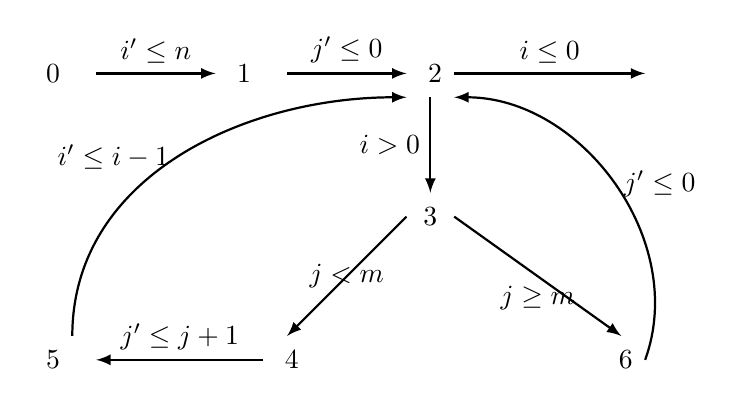
\begin{tikzpicture}[scale=\textwidth/20cm,samples=200]
    \draw[] (-8, 10) circle (0pt) node{{ $0$}};
    \draw[] (-4, 10) circle (0pt) node{{ $1$}};
    \draw[] (0, 10) circle (0pt) node{{ $2$}};
    \draw[] (0, 7) circle (0pt) node{{$3$}};
    \draw[] (-3, 4) circle (0pt) node{{ $4$}};
    \draw[] (-8, 4) circle (0pt) node{{ $5$}};
    \draw[] (4, 4) circle (0pt) node{{ $6$}};
    % Counter Variables
    \draw[] (5, 10) circle (0pt) node {\textbf{$\lex$}};
    %
    % Control Flow Edges:
    \draw[ thick, -latex] (-7, 10)  -- node [above] {$i' \leq n$}(-4.5, 10);
    \draw[ thick, -latex] (-3, 10)  -- node [above] {$j' \leq 0$}(-0.5, 10);
    \draw[ thick, -latex] (0, 9.5)  -- node [left] {$i > 0$} (0, 7.5) ;
    \draw[ thick, -latex] (0.5, 7)  -- node [below] {$ j \geq m $}  (4, 4.5);
    \draw[ thick, -latex] (-7.5, 4.5)  to  [out=90,in=180]  node [left] {$i' \leq i - 1$ }(-0.5, 9.5);
    \draw[ thick, -latex] (4.5, 4)  to  [out=70,in=0]   node [right] {$j' \leq 0 $}(0.5, 9.5);
    \draw[ thick, -latex]  (-0.5, 7) -- node  {$j < m$}  (-3, 4.5) ;
    \draw[ thick, -latex]  (-3.5, 4) -- node [above] {$j' \leq j + 1$}  (-7, 4) ;
    \draw[ thick, -latex] (0.5, 10)  -- node [above] {$i \leq 0$}  (4.5, 10);
  \end{tikzpicture}
        \caption{}
\end{centering}
\end{subfigure}
{\small
\begin{subfigure}{.3\textwidth}
\begin{centering}
        $\tpath_0 = 0 \to 1 \to 2$ \\
        $\tpath_2 = 2 \to 3 \to 6 \to 2$ \\ 
        $\tpath_1 = 2 \to 3 \to 4 \to 5 \to 2$ \\
        $\tpath_3 = 2 \to \lex$
        \caption{}
\end{centering}
\end{subfigure}
}
{\small
\begin{subfigure}{.8\textwidth}
\begin{centering}
    $
    \tpath_0 ; 
    \rpchoose{2: \rprepeat(\rprepeat(\tpath_1); \tpath_2), 
    2: \rprepeat(\tpath_1)}; \tpath_3.
    $
\end{centering}
\end{subfigure}
}
\end{subfigure}
\vspace{-0.2cm}
\caption{
    (a) The two paths loop example,
    (b) the Abstract Transition Graph for $\kw{twoPathsWhile}(n, m)$,
    (c) the Simple Transition Paths of $\kw{twoPathsWhile}(n, m)$.}
    \vspace{-0.5cm}
        \label{fig:whileTwoCounters-overview}
    \end{figure}
    }



% Though we can use it as the \emph{reachability-bound} for location $1$ and $2$,
% the \emph{reachability-bounds} for control locations $4, 5$ and $6$ are still unclear.
To know the bounds for locations on different branches of a loop, 
it is necessary to know the alternative iteration patterns of the two paths.
So over its abstract transition graph generated by Section~\ref{sec:progabs} as Figure~\ref{fig:whileTwoCounters-overview}(b), we collect all its simple transition path as in Figure~\ref{fig:whileTwoCounters-overview}(c).
Then we transform the loop by explicitly computing the interleaving between paths and
%  using the control-flow refinement technique from~\cite{GulwaniJK09} and 
generates a refined program $\rprog$ as the bottom part of Figure~\ref{fig:whileTwoCounters-overview}.
% % 
% % The refined program for program $\kw{twoPathsWhile}$ is
% % \[
%   $
%   \tpath_0 ; 
%   \rpchoose{2: \rprepeat_2(\rprepeat_1(\tpath_1); \tpath_2), 
%   2: \rprepeat_1(\tpath_1)}; \tpath_3.
%   $
% % \]
From this refined program, we can explicitly tell two possible path interleaving patterns.
In the first one, $\tpath_2$ will be executed after all the iterations of $\tpath_1$ are done, and in the second one,
the entire loop is done after $\tpath_1$ finish the iteration.
Then the following computation based on this refined program can compute more accurate reachability-bounds.
\end{example}
